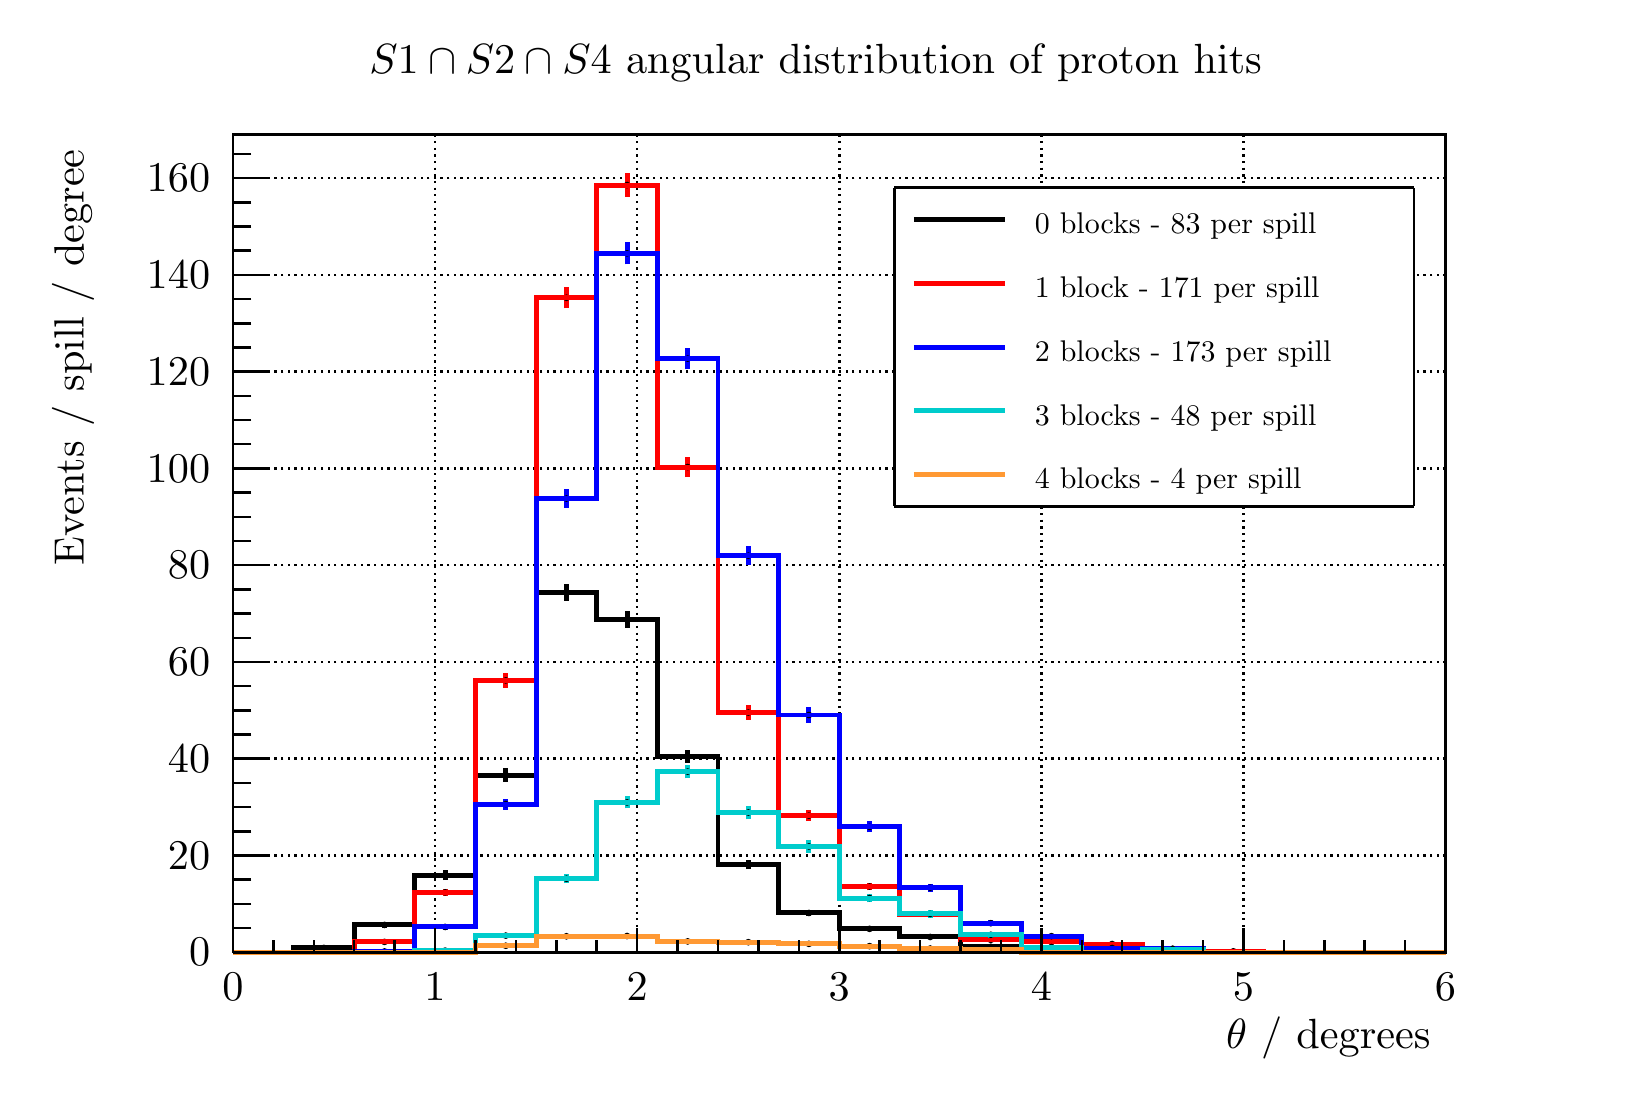
\begin{tikzpicture}
\pgfdeclareplotmark{cross} {
\pgfpathmoveto{\pgfpoint{-0.3\pgfplotmarksize}{\pgfplotmarksize}}
\pgfpathlineto{\pgfpoint{+0.3\pgfplotmarksize}{\pgfplotmarksize}}
\pgfpathlineto{\pgfpoint{+0.3\pgfplotmarksize}{0.3\pgfplotmarksize}}
\pgfpathlineto{\pgfpoint{+1\pgfplotmarksize}{0.3\pgfplotmarksize}}
\pgfpathlineto{\pgfpoint{+1\pgfplotmarksize}{-0.3\pgfplotmarksize}}
\pgfpathlineto{\pgfpoint{+0.3\pgfplotmarksize}{-0.3\pgfplotmarksize}}
\pgfpathlineto{\pgfpoint{+0.3\pgfplotmarksize}{-1.\pgfplotmarksize}}
\pgfpathlineto{\pgfpoint{-0.3\pgfplotmarksize}{-1.\pgfplotmarksize}}
\pgfpathlineto{\pgfpoint{-0.3\pgfplotmarksize}{-0.3\pgfplotmarksize}}
\pgfpathlineto{\pgfpoint{-1.\pgfplotmarksize}{-0.3\pgfplotmarksize}}
\pgfpathlineto{\pgfpoint{-1.\pgfplotmarksize}{0.3\pgfplotmarksize}}
\pgfpathlineto{\pgfpoint{-0.3\pgfplotmarksize}{0.3\pgfplotmarksize}}
\pgfpathclose
\pgfusepathqstroke
}
\pgfdeclareplotmark{cross*} {
\pgfpathmoveto{\pgfpoint{-0.3\pgfplotmarksize}{\pgfplotmarksize}}
\pgfpathlineto{\pgfpoint{+0.3\pgfplotmarksize}{\pgfplotmarksize}}
\pgfpathlineto{\pgfpoint{+0.3\pgfplotmarksize}{0.3\pgfplotmarksize}}
\pgfpathlineto{\pgfpoint{+1\pgfplotmarksize}{0.3\pgfplotmarksize}}
\pgfpathlineto{\pgfpoint{+1\pgfplotmarksize}{-0.3\pgfplotmarksize}}
\pgfpathlineto{\pgfpoint{+0.3\pgfplotmarksize}{-0.3\pgfplotmarksize}}
\pgfpathlineto{\pgfpoint{+0.3\pgfplotmarksize}{-1.\pgfplotmarksize}}
\pgfpathlineto{\pgfpoint{-0.3\pgfplotmarksize}{-1.\pgfplotmarksize}}
\pgfpathlineto{\pgfpoint{-0.3\pgfplotmarksize}{-0.3\pgfplotmarksize}}
\pgfpathlineto{\pgfpoint{-1.\pgfplotmarksize}{-0.3\pgfplotmarksize}}
\pgfpathlineto{\pgfpoint{-1.\pgfplotmarksize}{0.3\pgfplotmarksize}}
\pgfpathlineto{\pgfpoint{-0.3\pgfplotmarksize}{0.3\pgfplotmarksize}}
\pgfpathclose
\pgfusepathqfillstroke
}
\pgfdeclareplotmark{newstar} {
\pgfpathmoveto{\pgfqpoint{0pt}{\pgfplotmarksize}}
\pgfpathlineto{\pgfqpointpolar{44}{0.5\pgfplotmarksize}}
\pgfpathlineto{\pgfqpointpolar{18}{\pgfplotmarksize}}
\pgfpathlineto{\pgfqpointpolar{-20}{0.5\pgfplotmarksize}}
\pgfpathlineto{\pgfqpointpolar{-54}{\pgfplotmarksize}}
\pgfpathlineto{\pgfqpointpolar{-90}{0.5\pgfplotmarksize}}
\pgfpathlineto{\pgfqpointpolar{234}{\pgfplotmarksize}}
\pgfpathlineto{\pgfqpointpolar{198}{0.5\pgfplotmarksize}}
\pgfpathlineto{\pgfqpointpolar{162}{\pgfplotmarksize}}
\pgfpathlineto{\pgfqpointpolar{134}{0.5\pgfplotmarksize}}
\pgfpathclose
\pgfusepathqstroke
}
\pgfdeclareplotmark{newstar*} {
\pgfpathmoveto{\pgfqpoint{0pt}{\pgfplotmarksize}}
\pgfpathlineto{\pgfqpointpolar{44}{0.5\pgfplotmarksize}}
\pgfpathlineto{\pgfqpointpolar{18}{\pgfplotmarksize}}
\pgfpathlineto{\pgfqpointpolar{-20}{0.5\pgfplotmarksize}}
\pgfpathlineto{\pgfqpointpolar{-54}{\pgfplotmarksize}}
\pgfpathlineto{\pgfqpointpolar{-90}{0.5\pgfplotmarksize}}
\pgfpathlineto{\pgfqpointpolar{234}{\pgfplotmarksize}}
\pgfpathlineto{\pgfqpointpolar{198}{0.5\pgfplotmarksize}}
\pgfpathlineto{\pgfqpointpolar{162}{\pgfplotmarksize}}
\pgfpathlineto{\pgfqpointpolar{134}{0.5\pgfplotmarksize}}
\pgfpathclose
\pgfusepathqfillstroke
}
\definecolor{c}{rgb}{1,1,1};
\draw [color=c, fill=c] (0,0) rectangle (20,13.4957);
\draw [color=c, fill=c] (2.6,1.75444) rectangle (18,12.1461);
\definecolor{c}{rgb}{0,0,0};
\draw [c,line width=0.9] (2.6,1.75444) -- (2.6,12.1461) -- (18,12.1461) -- (18,1.75444) -- (2.6,1.75444);
\definecolor{c}{rgb}{1,1,1};
\draw [color=c, fill=c] (2.6,1.75444) rectangle (18,12.1461);
\definecolor{c}{rgb}{0,0,0};
\draw [c,line width=0.9] (2.6,1.75444) -- (2.6,12.1461) -- (18,12.1461) -- (18,1.75444) -- (2.6,1.75444);
\draw [c,line width=0.9] (2.6,1.75444) -- (18,1.75444);
\draw [c,dash pattern=on 0.80pt off 1.60pt ,line width=0.9] (2.6,12.1461) -- (2.6,1.75444);
\draw [c,dash pattern=on 0.80pt off 1.60pt ,line width=0.9] (5.16667,12.1461) -- (5.16667,1.75444);
\draw [c,dash pattern=on 0.80pt off 1.60pt ,line width=0.9] (7.73333,12.1461) -- (7.73333,1.75444);
\draw [c,dash pattern=on 0.80pt off 1.60pt ,line width=0.9] (10.3,12.1461) -- (10.3,1.75444);
\draw [c,dash pattern=on 0.80pt off 1.60pt ,line width=0.9] (12.8667,12.1461) -- (12.8667,1.75444);
\draw [c,dash pattern=on 0.80pt off 1.60pt ,line width=0.9] (15.4333,12.1461) -- (15.4333,1.75444);
\draw [c,dash pattern=on 0.80pt off 1.60pt ,line width=0.9] (18,12.1461) -- (18,1.75444);
\draw [c,line width=0.9] (2.6,1.75444) -- (2.6,12.1461);
\draw [c,dash pattern=on 0.80pt off 1.60pt ,line width=0.9] (18,1.76093) -- (2.6,1.76093);
\draw [c,dash pattern=on 0.80pt off 1.60pt ,line width=0.9] (18,2.98973) -- (2.6,2.98973);
\draw [c,dash pattern=on 0.80pt off 1.60pt ,line width=0.9] (18,4.21853) -- (2.6,4.21853);
\draw [c,dash pattern=on 0.80pt off 1.60pt ,line width=0.9] (18,5.44733) -- (2.6,5.44733);
\draw [c,dash pattern=on 0.80pt off 1.60pt ,line width=0.9] (18,6.67614) -- (2.6,6.67614);
\draw [c,dash pattern=on 0.80pt off 1.60pt ,line width=0.9] (18,7.90494) -- (2.6,7.90494);
\draw [c,dash pattern=on 0.80pt off 1.60pt ,line width=0.9] (18,9.13374) -- (2.6,9.13374);
\draw [c,dash pattern=on 0.80pt off 1.60pt ,line width=0.9] (18,10.3625) -- (2.6,10.3625);
\draw [c,dash pattern=on 0.80pt off 1.60pt ,line width=0.9] (18,11.5913) -- (2.6,11.5913);
\draw [c,dash pattern=on 0.80pt off 1.60pt ,line width=0.9] (18,1.76093) -- (2.6,1.76093);
\draw [c,dash pattern=on 0.80pt off 1.60pt ,line width=0.9] (18,11.5913) -- (2.6,11.5913);
\definecolor{c}{rgb}{0,0,0.6};
\draw [c,line width=0.9] (2.6,1.76093) -- (3.37,1.76093) -- (3.37,1.76093) -- (4.14,1.76093) -- (4.14,1.76093) -- (4.91,1.76093) -- (4.91,1.76093) -- (5.68,1.76093) -- (5.68,1.76093) -- (6.45,1.76093) -- (6.45,1.76093) -- (7.22,1.76093) --
 (7.22,1.76093) -- (7.99,1.76093) -- (7.99,1.76093) -- (8.76,1.76093) -- (8.76,1.76093) -- (9.53,1.76093) -- (9.53,1.76093) -- (10.3,1.76093) -- (10.3,1.76093) -- (11.07,1.76093) -- (11.07,1.76093) -- (11.84,1.76093) -- (11.84,1.76093) --
 (12.61,1.76093) -- (12.61,1.76093) -- (13.38,1.76093) -- (13.38,1.76093) -- (14.15,1.76093) -- (14.15,1.76093) -- (14.92,1.76093) -- (14.92,1.76093) -- (15.69,1.76093) -- (15.69,1.76093) -- (16.46,1.76093) -- (16.46,1.76093) -- (17.23,1.76093) --
 (17.23,1.76093) -- (18,1.76093);
\definecolor{c}{rgb}{0,0,0};
\draw [c,line width=0.9] (2.6,1.75444) -- (18,1.75444);
\draw [c,line width=0.9] (2.6,2.06619) -- (2.6,1.75444);
\draw [c,line width=0.9] (3.11333,1.91032) -- (3.11333,1.75444);
\draw [c,line width=0.9] (3.62667,1.91032) -- (3.62667,1.75444);
\draw [c,line width=0.9] (4.14,1.91032) -- (4.14,1.75444);
\draw [c,line width=0.9] (4.65333,1.91032) -- (4.65333,1.75444);
\draw [c,line width=0.9] (5.16667,2.06619) -- (5.16667,1.75444);
\draw [c,line width=0.9] (5.68,1.91032) -- (5.68,1.75444);
\draw [c,line width=0.9] (6.19333,1.91032) -- (6.19333,1.75444);
\draw [c,line width=0.9] (6.70667,1.91032) -- (6.70667,1.75444);
\draw [c,line width=0.9] (7.22,1.91032) -- (7.22,1.75444);
\draw [c,line width=0.9] (7.73333,2.06619) -- (7.73333,1.75444);
\draw [c,line width=0.9] (8.24667,1.91032) -- (8.24667,1.75444);
\draw [c,line width=0.9] (8.76,1.91032) -- (8.76,1.75444);
\draw [c,line width=0.9] (9.27333,1.91032) -- (9.27333,1.75444);
\draw [c,line width=0.9] (9.78667,1.91032) -- (9.78667,1.75444);
\draw [c,line width=0.9] (10.3,2.06619) -- (10.3,1.75444);
\draw [c,line width=0.9] (10.8133,1.91032) -- (10.8133,1.75444);
\draw [c,line width=0.9] (11.3267,1.91032) -- (11.3267,1.75444);
\draw [c,line width=0.9] (11.84,1.91032) -- (11.84,1.75444);
\draw [c,line width=0.9] (12.3533,1.91032) -- (12.3533,1.75444);
\draw [c,line width=0.9] (12.8667,2.06619) -- (12.8667,1.75444);
\draw [c,line width=0.9] (13.38,1.91032) -- (13.38,1.75444);
\draw [c,line width=0.9] (13.8933,1.91032) -- (13.8933,1.75444);
\draw [c,line width=0.9] (14.4067,1.91032) -- (14.4067,1.75444);
\draw [c,line width=0.9] (14.92,1.91032) -- (14.92,1.75444);
\draw [c,line width=0.9] (15.4333,2.06619) -- (15.4333,1.75444);
\draw [c,line width=0.9] (15.9467,1.91032) -- (15.9467,1.75444);
\draw [c,line width=0.9] (16.46,1.91032) -- (16.46,1.75444);
\draw [c,line width=0.9] (16.9733,1.91032) -- (16.9733,1.75444);
\draw [c,line width=0.9] (17.4867,1.91032) -- (17.4867,1.75444);
\draw [c,line width=0.9] (18,2.06619) -- (18,1.75444);
\draw [anchor=base] (2.6,1.14713) node[scale=1.52731, color=c, rotate=0]{0};
\draw [anchor=base] (5.16667,1.14713) node[scale=1.52731, color=c, rotate=0]{1};
\draw [anchor=base] (7.73333,1.14713) node[scale=1.52731, color=c, rotate=0]{2};
\draw [anchor=base] (10.3,1.14713) node[scale=1.52731, color=c, rotate=0]{3};
\draw [anchor=base] (12.8667,1.14713) node[scale=1.52731, color=c, rotate=0]{4};
\draw [anchor=base] (15.4333,1.14713) node[scale=1.52731, color=c, rotate=0]{5};
\draw [anchor=base] (18,1.14713) node[scale=1.52731, color=c, rotate=0]{6};
\draw [anchor= east] (18,0.674785) node[scale=1.52731, color=c, rotate=0]{$\theta$ / degrees};
\draw [c,line width=0.9] (2.6,1.75444) -- (2.6,12.1461);
\draw [c,line width=0.9] (3.062,1.76093) -- (2.6,1.76093);
\draw [c,line width=0.9] (2.831,2.06813) -- (2.6,2.06813);
\draw [c,line width=0.9] (2.831,2.37533) -- (2.6,2.37533);
\draw [c,line width=0.9] (2.831,2.68253) -- (2.6,2.68253);
\draw [c,line width=0.9] (3.062,2.98973) -- (2.6,2.98973);
\draw [c,line width=0.9] (2.831,3.29693) -- (2.6,3.29693);
\draw [c,line width=0.9] (2.831,3.60413) -- (2.6,3.60413);
\draw [c,line width=0.9] (2.831,3.91133) -- (2.6,3.91133);
\draw [c,line width=0.9] (3.062,4.21853) -- (2.6,4.21853);
\draw [c,line width=0.9] (2.831,4.52573) -- (2.6,4.52573);
\draw [c,line width=0.9] (2.831,4.83293) -- (2.6,4.83293);
\draw [c,line width=0.9] (2.831,5.14013) -- (2.6,5.14013);
\draw [c,line width=0.9] (3.062,5.44733) -- (2.6,5.44733);
\draw [c,line width=0.9] (2.831,5.75454) -- (2.6,5.75454);
\draw [c,line width=0.9] (2.831,6.06174) -- (2.6,6.06174);
\draw [c,line width=0.9] (2.831,6.36894) -- (2.6,6.36894);
\draw [c,line width=0.9] (3.062,6.67614) -- (2.6,6.67614);
\draw [c,line width=0.9] (2.831,6.98334) -- (2.6,6.98334);
\draw [c,line width=0.9] (2.831,7.29054) -- (2.6,7.29054);
\draw [c,line width=0.9] (2.831,7.59774) -- (2.6,7.59774);
\draw [c,line width=0.9] (3.062,7.90494) -- (2.6,7.90494);
\draw [c,line width=0.9] (2.831,8.21214) -- (2.6,8.21214);
\draw [c,line width=0.9] (2.831,8.51934) -- (2.6,8.51934);
\draw [c,line width=0.9] (2.831,8.82654) -- (2.6,8.82654);
\draw [c,line width=0.9] (3.062,9.13374) -- (2.6,9.13374);
\draw [c,line width=0.9] (2.831,9.44094) -- (2.6,9.44094);
\draw [c,line width=0.9] (2.831,9.74814) -- (2.6,9.74814);
\draw [c,line width=0.9] (2.831,10.0553) -- (2.6,10.0553);
\draw [c,line width=0.9] (3.062,10.3625) -- (2.6,10.3625);
\draw [c,line width=0.9] (2.831,10.6697) -- (2.6,10.6697);
\draw [c,line width=0.9] (2.831,10.9769) -- (2.6,10.9769);
\draw [c,line width=0.9] (2.831,11.2841) -- (2.6,11.2841);
\draw [c,line width=0.9] (3.062,11.5913) -- (2.6,11.5913);
\draw [c,line width=0.9] (3.062,1.76093) -- (2.6,1.76093);
\draw [c,line width=0.9] (3.062,11.5913) -- (2.6,11.5913);
\draw [c,line width=0.9] (2.831,11.8985) -- (2.6,11.8985);
\draw [anchor= east] (2.5,1.76093) node[scale=1.52731, color=c, rotate=0]{0};
\draw [anchor= east] (2.5,2.98973) node[scale=1.52731, color=c, rotate=0]{20};
\draw [anchor= east] (2.5,4.21853) node[scale=1.52731, color=c, rotate=0]{40};
\draw [anchor= east] (2.5,5.44733) node[scale=1.52731, color=c, rotate=0]{60};
\draw [anchor= east] (2.5,6.67614) node[scale=1.52731, color=c, rotate=0]{80};
\draw [anchor= east] (2.5,7.90494) node[scale=1.52731, color=c, rotate=0]{100};
\draw [anchor= east] (2.5,9.13374) node[scale=1.52731, color=c, rotate=0]{120};
\draw [anchor= east] (2.5,10.3625) node[scale=1.52731, color=c, rotate=0]{140};
\draw [anchor= east] (2.5,11.5913) node[scale=1.52731, color=c, rotate=0]{160};
\draw [anchor= east] (0.568481,12.1461) node[scale=1.52731, color=c, rotate=90]{Events / spill / degree};
\draw [c,line width=1.8] (3.755,1.79762) -- (3.755,1.81604);
\draw [c,line width=1.8] (3.755,1.81604) -- (3.755,1.83446);
\foreach \P in {(3.755,1.81604)}{\draw[mark options={color=c,fill=c},mark size=2.402402pt,mark=*,mark size=1pt] plot coordinates {\P};}
\draw [c,line width=1.8] (4.525,2.06705) -- (4.525,2.10782);
\draw [c,line width=1.8] (4.525,2.10782) -- (4.525,2.1486);
\foreach \P in {(4.525,2.10782)}{\draw[mark options={color=c,fill=c},mark size=2.402402pt,mark=*,mark size=1pt] plot coordinates {\P};}
\draw [c,line width=1.8] (5.295,2.6764) -- (5.295,2.73838);
\draw [c,line width=1.8] (5.295,2.73838) -- (5.295,2.80036);
\foreach \P in {(5.295,2.73838)}{\draw[mark options={color=c,fill=c},mark size=2.402402pt,mark=*,mark size=1pt] plot coordinates {\P};}
\draw [c,line width=1.8] (6.065,3.92747) -- (6.065,4.01129);
\draw [c,line width=1.8] (6.065,4.01129) -- (6.065,4.09512);
\foreach \P in {(6.065,4.01129)}{\draw[mark options={color=c,fill=c},mark size=2.402402pt,mark=*,mark size=1pt] plot coordinates {\P};}
\draw [c,line width=1.8] (6.835,6.22429) -- (6.835,6.33134);
\draw [c,line width=1.8] (6.835,6.33134) -- (6.835,6.43839);
\foreach \P in {(6.835,6.33134)}{\draw[mark options={color=c,fill=c},mark size=2.402402pt,mark=*,mark size=1pt] plot coordinates {\P};}
\draw [c,line width=1.8] (7.605,5.88431) -- (7.605,5.98662);
\draw [c,line width=1.8] (7.605,5.98662) -- (7.605,6.08893);
\foreach \P in {(7.605,5.98662)}{\draw[mark options={color=c,fill=c},mark size=2.402402pt,mark=*,mark size=1pt] plot coordinates {\P};}
\draw [c,line width=1.8] (8.375,4.16304) -- (8.375,4.24479);
\draw [c,line width=1.8] (8.375,4.24479) -- (8.375,4.32653);
\foreach \P in {(8.375,4.24479)}{\draw[mark options={color=c,fill=c},mark size=2.402402pt,mark=*,mark size=1pt] plot coordinates {\P};}
\draw [c,line width=1.8] (9.145,2.81619) -- (9.145,2.87253);
\draw [c,line width=1.8] (9.145,2.87253) -- (9.145,2.92887);
\foreach \P in {(9.145,2.87253)}{\draw[mark options={color=c,fill=c},mark size=2.402402pt,mark=*,mark size=1pt] plot coordinates {\P};}
\draw [c,line width=1.8] (9.915,2.22128) -- (9.915,2.25961);
\draw [c,line width=1.8] (9.915,2.25961) -- (9.915,2.29794);
\foreach \P in {(9.915,2.25961)}{\draw[mark options={color=c,fill=c},mark size=2.402402pt,mark=*,mark size=1pt] plot coordinates {\P};}
\draw [c,line width=1.8] (10.685,2.02747) -- (10.685,2.05774);
\draw [c,line width=1.8] (10.685,2.05774) -- (10.685,2.088);
\foreach \P in {(10.685,2.05774)}{\draw[mark options={color=c,fill=c},mark size=2.402402pt,mark=*,mark size=1pt] plot coordinates {\P};}
\draw [c,line width=1.8] (11.455,1.93051) -- (11.455,1.95456);
\draw [c,line width=1.8] (11.455,1.95456) -- (11.455,1.97862);
\foreach \P in {(11.455,1.95456)}{\draw[mark options={color=c,fill=c},mark size=2.402402pt,mark=*,mark size=1pt] plot coordinates {\P};}
\draw [c,line width=1.8] (12.225,1.81447) -- (12.225,1.82988);
\draw [c,line width=1.8] (12.225,1.82988) -- (12.225,1.84529);
\foreach \P in {(12.225,1.82988)}{\draw[mark options={color=c,fill=c},mark size=2.402402pt,mark=*,mark size=1pt] plot coordinates {\P};}
\draw [c,line width=1.8] (12.995,1.79777) -- (12.995,1.81151);
\draw [c,line width=1.8] (12.995,1.81151) -- (12.995,1.82525);
\foreach \P in {(12.995,1.81151)}{\draw[mark options={color=c,fill=c},mark size=2.402402pt,mark=*,mark size=1pt] plot coordinates {\P};}
\draw [c,line width=1.8] (13.765,1.76838) -- (13.765,1.77856);
\draw [c,line width=1.8] (13.765,1.77856) -- (13.765,1.78873);
\foreach \P in {(13.765,1.77856)}{\draw[mark options={color=c,fill=c},mark size=2.402402pt,mark=*,mark size=1pt] plot coordinates {\P};}
\draw [c,line width=1.8] (14.535,1.77475) -- (14.535,1.7871);
\draw [c,line width=1.8] (14.535,1.7871) -- (14.535,1.79945);
\foreach \P in {(14.535,1.7871)}{\draw[mark options={color=c,fill=c},mark size=2.402402pt,mark=*,mark size=1pt] plot coordinates {\P};}
\draw [c,line width=1.8] (2.6,1.76093) -- (3.37,1.76093) -- (3.37,1.81604) -- (4.14,1.81604) -- (4.14,2.10782) -- (4.91,2.10782) -- (4.91,2.73838) -- (5.68,2.73838) -- (5.68,4.01129) -- (6.45,4.01129) -- (6.45,6.33134) -- (7.22,6.33134) --
 (7.22,5.98662) -- (7.99,5.98662) -- (7.99,4.24479) -- (8.76,4.24479) -- (8.76,2.87253) -- (9.53,2.87253) -- (9.53,2.25961) -- (10.3,2.25961) -- (10.3,2.05774) -- (11.07,2.05774) -- (11.07,1.95456) -- (11.84,1.95456) -- (11.84,1.82988) --
 (12.61,1.82988) -- (12.61,1.81151) -- (13.38,1.81151) -- (13.38,1.77856) -- (14.15,1.77856) -- (14.15,1.7871) -- (14.92,1.7871) -- (14.92,1.76093) -- (15.69,1.76093) -- (15.69,1.76093) -- (16.46,1.76093) -- (16.46,1.76093) -- (17.23,1.76093) --
 (17.23,1.76093) -- (18,1.76093);
\definecolor{c}{rgb}{1,0,0};
\draw [c,line width=1.8] (4.525,1.87027) -- (4.525,1.8923);
\draw [c,line width=1.8] (4.525,1.8923) -- (4.525,1.91434);
\definecolor{c}{rgb}{0,0,0};
\foreach \P in {(4.525,1.8923)}{\draw[mark options={color=c,fill=c},mark size=2.402402pt,mark=*,mark size=1pt] plot coordinates {\P};}
\definecolor{c}{rgb}{1,0,0};
\draw [c,line width=1.8] (5.295,2.47603) -- (5.295,2.52118);
\draw [c,line width=1.8] (5.295,2.52118) -- (5.295,2.56633);
\definecolor{c}{rgb}{0,0,0};
\foreach \P in {(5.295,2.52118)}{\draw[mark options={color=c,fill=c},mark size=2.402402pt,mark=*,mark size=1pt] plot coordinates {\P};}
\definecolor{c}{rgb}{1,0,0};
\draw [c,line width=1.8] (6.065,5.12195) -- (6.065,5.21308);
\draw [c,line width=1.8] (6.065,5.21308) -- (6.065,5.30421);
\definecolor{c}{rgb}{0,0,0};
\foreach \P in {(6.065,5.21308)}{\draw[mark options={color=c,fill=c},mark size=2.402402pt,mark=*,mark size=1pt] plot coordinates {\P};}
\definecolor{c}{rgb}{1,0,0};
\draw [c,line width=1.8] (6.835,9.93852) -- (6.835,10.0725);
\draw [c,line width=1.8] (6.835,10.0725) -- (6.835,10.2065);
\definecolor{c}{rgb}{0,0,0};
\foreach \P in {(6.835,10.0725)}{\draw[mark options={color=c,fill=c},mark size=2.402402pt,mark=*,mark size=1pt] plot coordinates {\P};}
\definecolor{c}{rgb}{1,0,0};
\draw [c,line width=1.8] (7.605,11.3567) -- (7.605,11.5041);
\draw [c,line width=1.8] (7.605,11.5041) -- (7.605,11.6516);
\definecolor{c}{rgb}{0,0,0};
\foreach \P in {(7.605,11.5041)}{\draw[mark options={color=c,fill=c},mark size=2.402402pt,mark=*,mark size=1pt] plot coordinates {\P};}
\definecolor{c}{rgb}{1,0,0};
\draw [c,line width=1.8] (8.375,7.79539) -- (8.375,7.92254);
\draw [c,line width=1.8] (8.375,7.92254) -- (8.375,8.0497);
\definecolor{c}{rgb}{0,0,0};
\foreach \P in {(8.375,7.92254)}{\draw[mark options={color=c,fill=c},mark size=2.402402pt,mark=*,mark size=1pt] plot coordinates {\P};}
\definecolor{c}{rgb}{1,0,0};
\draw [c,line width=1.8] (9.145,4.71262) -- (9.145,4.80477);
\draw [c,line width=1.8] (9.145,4.80477) -- (9.145,4.89691);
\definecolor{c}{rgb}{0,0,0};
\foreach \P in {(9.145,4.80477)}{\draw[mark options={color=c,fill=c},mark size=2.402402pt,mark=*,mark size=1pt] plot coordinates {\P};}
\definecolor{c}{rgb}{1,0,0};
\draw [c,line width=1.8] (9.915,3.42476) -- (9.915,3.49539);
\draw [c,line width=1.8] (9.915,3.49539) -- (9.915,3.56602);
\definecolor{c}{rgb}{0,0,0};
\foreach \P in {(9.915,3.49539)}{\draw[mark options={color=c,fill=c},mark size=2.402402pt,mark=*,mark size=1pt] plot coordinates {\P};}
\definecolor{c}{rgb}{1,0,0};
\draw [c,line width=1.8] (10.685,2.54579) -- (10.685,2.59582);
\draw [c,line width=1.8] (10.685,2.59582) -- (10.685,2.64585);
\definecolor{c}{rgb}{0,0,0};
\foreach \P in {(10.685,2.59582)}{\draw[mark options={color=c,fill=c},mark size=2.402402pt,mark=*,mark size=1pt] plot coordinates {\P};}
\definecolor{c}{rgb}{1,0,0};
\draw [c,line width=1.8] (11.455,2.20106) -- (11.455,2.24056);
\draw [c,line width=1.8] (11.455,2.24056) -- (11.455,2.28006);
\definecolor{c}{rgb}{0,0,0};
\foreach \P in {(11.455,2.24056)}{\draw[mark options={color=c,fill=c},mark size=2.402402pt,mark=*,mark size=1pt] plot coordinates {\P};}
\definecolor{c}{rgb}{1,0,0};
\draw [c,line width=1.8] (12.225,1.89565) -- (12.225,1.91791);
\draw [c,line width=1.8] (12.225,1.91791) -- (12.225,1.94017);
\definecolor{c}{rgb}{0,0,0};
\foreach \P in {(12.225,1.91791)}{\draw[mark options={color=c,fill=c},mark size=2.402402pt,mark=*,mark size=1pt] plot coordinates {\P};}
\definecolor{c}{rgb}{1,0,0};
\draw [c,line width=1.8] (12.995,1.87062) -- (12.995,1.8917);
\draw [c,line width=1.8] (12.995,1.8917) -- (12.995,1.91279);
\definecolor{c}{rgb}{0,0,0};
\foreach \P in {(12.995,1.8917)}{\draw[mark options={color=c,fill=c},mark size=2.402402pt,mark=*,mark size=1pt] plot coordinates {\P};}
\definecolor{c}{rgb}{1,0,0};
\draw [c,line width=1.8] (13.765,1.8444) -- (13.765,1.86468);
\draw [c,line width=1.8] (13.765,1.86468) -- (13.765,1.88497);
\definecolor{c}{rgb}{0,0,0};
\foreach \P in {(13.765,1.86468)}{\draw[mark options={color=c,fill=c},mark size=2.402402pt,mark=*,mark size=1pt] plot coordinates {\P};}
\definecolor{c}{rgb}{1,0,0};
\draw [c,line width=1.8] (14.535,1.78075) -- (14.535,1.79424);
\draw [c,line width=1.8] (14.535,1.79424) -- (14.535,1.80772);
\definecolor{c}{rgb}{0,0,0};
\foreach \P in {(14.535,1.79424)}{\draw[mark options={color=c,fill=c},mark size=2.402402pt,mark=*,mark size=1pt] plot coordinates {\P};}
\definecolor{c}{rgb}{1,0,0};
\draw [c,line width=1.8] (15.305,1.75863) -- (15.305,1.77229);
\draw [c,line width=1.8] (15.305,1.77229) -- (15.305,1.78596);
\definecolor{c}{rgb}{0,0,0};
\foreach \P in {(15.305,1.77229)}{\draw[mark options={color=c,fill=c},mark size=2.402402pt,mark=*,mark size=1pt] plot coordinates {\P};}
\definecolor{c}{rgb}{1,0,0};
\draw [c,line width=1.8] (2.6,1.76093) -- (3.37,1.76093) -- (3.37,1.76093) -- (4.14,1.76093) -- (4.14,1.8923) -- (4.91,1.8923) -- (4.91,2.52118) -- (5.68,2.52118) -- (5.68,5.21308) -- (6.45,5.21308) -- (6.45,10.0725) -- (7.22,10.0725) --
 (7.22,11.5041) -- (7.99,11.5041) -- (7.99,7.92254) -- (8.76,7.92254) -- (8.76,4.80477) -- (9.53,4.80477) -- (9.53,3.49539) -- (10.3,3.49539) -- (10.3,2.59582) -- (11.07,2.59582) -- (11.07,2.24056) -- (11.84,2.24056) -- (11.84,1.91791) --
 (12.61,1.91791) -- (12.61,1.8917) -- (13.38,1.8917) -- (13.38,1.86468) -- (14.15,1.86468) -- (14.15,1.79424) -- (14.92,1.79424) -- (14.92,1.77229) -- (15.69,1.77229) -- (15.69,1.76093) -- (16.46,1.76093) -- (16.46,1.76093) -- (17.23,1.76093) --
 (17.23,1.76093) -- (18,1.76093);
\definecolor{c}{rgb}{0,0,1};
\draw [c,line width=1.8] (4.525,1.75444) -- (4.525,1.77105);
\draw [c,line width=1.8] (4.525,1.77105) -- (4.525,1.78766);
\definecolor{c}{rgb}{0,0,0};
\foreach \P in {(4.525,1.77105)}{\draw[mark options={color=c,fill=c},mark size=2.402402pt,mark=*,mark size=1pt] plot coordinates {\P};}
\definecolor{c}{rgb}{0,0,1};
\draw [c,line width=1.8] (5.295,2.04936) -- (5.295,2.08221);
\draw [c,line width=1.8] (5.295,2.08221) -- (5.295,2.11507);
\definecolor{c}{rgb}{0,0,0};
\foreach \P in {(5.295,2.08221)}{\draw[mark options={color=c,fill=c},mark size=2.402402pt,mark=*,mark size=1pt] plot coordinates {\P};}
\definecolor{c}{rgb}{0,0,1};
\draw [c,line width=1.8] (6.065,3.57135) -- (6.065,3.64214);
\draw [c,line width=1.8] (6.065,3.64214) -- (6.065,3.71292);
\definecolor{c}{rgb}{0,0,0};
\foreach \P in {(6.065,3.64214)}{\draw[mark options={color=c,fill=c},mark size=2.402402pt,mark=*,mark size=1pt] plot coordinates {\P};}
\definecolor{c}{rgb}{0,0,1};
\draw [c,line width=1.8] (6.835,7.40577) -- (6.835,7.52278);
\draw [c,line width=1.8] (6.835,7.52278) -- (6.835,7.63978);
\definecolor{c}{rgb}{0,0,0};
\foreach \P in {(6.835,7.52278)}{\draw[mark options={color=c,fill=c},mark size=2.402402pt,mark=*,mark size=1pt] plot coordinates {\P};}
\definecolor{c}{rgb}{0,0,1};
\draw [c,line width=1.8] (7.605,10.4954) -- (7.605,10.6362);
\draw [c,line width=1.8] (7.605,10.6362) -- (7.605,10.777);
\definecolor{c}{rgb}{0,0,0};
\foreach \P in {(7.605,10.6362)}{\draw[mark options={color=c,fill=c},mark size=2.402402pt,mark=*,mark size=1pt] plot coordinates {\P};}
\definecolor{c}{rgb}{0,0,1};
\draw [c,line width=1.8] (8.375,9.16191) -- (8.375,9.29976);
\draw [c,line width=1.8] (8.375,9.29976) -- (8.375,9.43761);
\definecolor{c}{rgb}{0,0,0};
\foreach \P in {(8.375,9.29976)}{\draw[mark options={color=c,fill=c},mark size=2.402402pt,mark=*,mark size=1pt] plot coordinates {\P};}
\definecolor{c}{rgb}{0,0,1};
\draw [c,line width=1.8] (9.145,6.67484) -- (9.145,6.79694);
\draw [c,line width=1.8] (9.145,6.79694) -- (9.145,6.91904);
\definecolor{c}{rgb}{0,0,0};
\foreach \P in {(9.145,6.79694)}{\draw[mark options={color=c,fill=c},mark size=2.402402pt,mark=*,mark size=1pt] plot coordinates {\P};}
\definecolor{c}{rgb}{0,0,1};
\draw [c,line width=1.8] (9.915,4.6775) -- (9.915,4.77358);
\draw [c,line width=1.8] (9.915,4.77358) -- (9.915,4.86966);
\definecolor{c}{rgb}{0,0,0};
\foreach \P in {(9.915,4.77358)}{\draw[mark options={color=c,fill=c},mark size=2.402402pt,mark=*,mark size=1pt] plot coordinates {\P};}
\definecolor{c}{rgb}{0,0,1};
\draw [c,line width=1.8] (10.685,3.28375) -- (10.685,3.35287);
\draw [c,line width=1.8] (10.685,3.35287) -- (10.685,3.422);
\definecolor{c}{rgb}{0,0,0};
\foreach \P in {(10.685,3.35287)}{\draw[mark options={color=c,fill=c},mark size=2.402402pt,mark=*,mark size=1pt] plot coordinates {\P};}
\definecolor{c}{rgb}{0,0,1};
\draw [c,line width=1.8] (11.455,2.52966) -- (11.455,2.5809);
\draw [c,line width=1.8] (11.455,2.5809) -- (11.455,2.63214);
\definecolor{c}{rgb}{0,0,0};
\foreach \P in {(11.455,2.5809)}{\draw[mark options={color=c,fill=c},mark size=2.402402pt,mark=*,mark size=1pt] plot coordinates {\P};}
\definecolor{c}{rgb}{0,0,1};
\draw [c,line width=1.8] (12.225,2.09368) -- (12.225,2.12933);
\draw [c,line width=1.8] (12.225,2.12933) -- (12.225,2.16497);
\definecolor{c}{rgb}{0,0,0};
\foreach \P in {(12.225,2.12933)}{\draw[mark options={color=c,fill=c},mark size=2.402402pt,mark=*,mark size=1pt] plot coordinates {\P};}
\definecolor{c}{rgb}{0,0,1};
\draw [c,line width=1.8] (12.995,1.93789) -- (12.995,1.96487);
\draw [c,line width=1.8] (12.995,1.96487) -- (12.995,1.99185);
\definecolor{c}{rgb}{0,0,0};
\foreach \P in {(12.995,1.96487)}{\draw[mark options={color=c,fill=c},mark size=2.402402pt,mark=*,mark size=1pt] plot coordinates {\P};}
\definecolor{c}{rgb}{0,0,1};
\draw [c,line width=1.8] (13.765,1.79522) -- (13.765,1.81389);
\draw [c,line width=1.8] (13.765,1.81389) -- (13.765,1.83256);
\definecolor{c}{rgb}{0,0,0};
\foreach \P in {(13.765,1.81389)}{\draw[mark options={color=c,fill=c},mark size=2.402402pt,mark=*,mark size=1pt] plot coordinates {\P};}
\definecolor{c}{rgb}{0,0,1};
\draw [c,line width=1.8] (14.535,1.78582) -- (14.535,1.80517);
\draw [c,line width=1.8] (14.535,1.80517) -- (14.535,1.82451);
\definecolor{c}{rgb}{0,0,0};
\foreach \P in {(14.535,1.80517)}{\draw[mark options={color=c,fill=c},mark size=2.402402pt,mark=*,mark size=1pt] plot coordinates {\P};}
\definecolor{c}{rgb}{0,0,1};
\draw [c,line width=1.8] (2.6,1.76093) -- (3.37,1.76093) -- (3.37,1.76093) -- (4.14,1.76093) -- (4.14,1.77105) -- (4.91,1.77105) -- (4.91,2.08221) -- (5.68,2.08221) -- (5.68,3.64214) -- (6.45,3.64214) -- (6.45,7.52278) -- (7.22,7.52278) --
 (7.22,10.6362) -- (7.99,10.6362) -- (7.99,9.29976) -- (8.76,9.29976) -- (8.76,6.79694) -- (9.53,6.79694) -- (9.53,4.77358) -- (10.3,4.77358) -- (10.3,3.35287) -- (11.07,3.35287) -- (11.07,2.5809) -- (11.84,2.5809) -- (11.84,2.12933) --
 (12.61,2.12933) -- (12.61,1.96487) -- (13.38,1.96487) -- (13.38,1.81389) -- (14.15,1.81389) -- (14.15,1.80517) -- (14.92,1.80517) -- (14.92,1.76093) -- (15.69,1.76093) -- (15.69,1.76093) -- (16.46,1.76093) -- (16.46,1.76093) -- (17.23,1.76093) --
 (17.23,1.76093) -- (18,1.76093);
\definecolor{c}{rgb}{0,0.8,0.8};
\draw [c,line width=1.8] (5.295,1.76346) -- (5.295,1.78112);
\draw [c,line width=1.8] (5.295,1.78112) -- (5.295,1.79877);
\definecolor{c}{rgb}{0,0,0};
\foreach \P in {(5.295,1.78112)}{\draw[mark options={color=c,fill=c},mark size=2.402402pt,mark=*,mark size=1pt] plot coordinates {\P};}
\definecolor{c}{rgb}{0,0.8,0.8};
\draw [c,line width=1.8] (6.065,1.94156) -- (6.065,1.97195);
\draw [c,line width=1.8] (6.065,1.97195) -- (6.065,2.00235);
\definecolor{c}{rgb}{0,0,0};
\foreach \P in {(6.065,1.97195)}{\draw[mark options={color=c,fill=c},mark size=2.402402pt,mark=*,mark size=1pt] plot coordinates {\P};}
\definecolor{c}{rgb}{0,0.8,0.8};
\draw [c,line width=1.8] (6.835,2.63552) -- (6.835,2.69389);
\draw [c,line width=1.8] (6.835,2.69389) -- (6.835,2.75225);
\definecolor{c}{rgb}{0,0,0};
\foreach \P in {(6.835,2.69389)}{\draw[mark options={color=c,fill=c},mark size=2.402402pt,mark=*,mark size=1pt] plot coordinates {\P};}
\definecolor{c}{rgb}{0,0.8,0.8};
\draw [c,line width=1.8] (7.605,3.58733) -- (7.605,3.66343);
\draw [c,line width=1.8] (7.605,3.66343) -- (7.605,3.73952);
\definecolor{c}{rgb}{0,0,0};
\foreach \P in {(7.605,3.66343)}{\draw[mark options={color=c,fill=c},mark size=2.402402pt,mark=*,mark size=1pt] plot coordinates {\P};}
\definecolor{c}{rgb}{0,0.8,0.8};
\draw [c,line width=1.8] (8.375,3.96797) -- (8.375,4.0547);
\draw [c,line width=1.8] (8.375,4.0547) -- (8.375,4.14143);
\definecolor{c}{rgb}{0,0,0};
\foreach \P in {(8.375,4.0547)}{\draw[mark options={color=c,fill=c},mark size=2.402402pt,mark=*,mark size=1pt] plot coordinates {\P};}
\definecolor{c}{rgb}{0,0.8,0.8};
\draw [c,line width=1.8] (9.145,3.44787) -- (9.145,3.53523);
\draw [c,line width=1.8] (9.145,3.53523) -- (9.145,3.62259);
\definecolor{c}{rgb}{0,0,0};
\foreach \P in {(9.145,3.53523)}{\draw[mark options={color=c,fill=c},mark size=2.402402pt,mark=*,mark size=1pt] plot coordinates {\P};}
\definecolor{c}{rgb}{0,0.8,0.8};
\draw [c,line width=1.8] (9.915,3.02309) -- (9.915,3.10414);
\draw [c,line width=1.8] (9.915,3.10414) -- (9.915,3.18518);
\definecolor{c}{rgb}{0,0,0};
\foreach \P in {(9.915,3.10414)}{\draw[mark options={color=c,fill=c},mark size=2.402402pt,mark=*,mark size=1pt] plot coordinates {\P};}
\definecolor{c}{rgb}{0,0.8,0.8};
\draw [c,line width=1.8] (10.685,2.39386) -- (10.685,2.44942);
\draw [c,line width=1.8] (10.685,2.44942) -- (10.685,2.50499);
\definecolor{c}{rgb}{0,0,0};
\foreach \P in {(10.685,2.44942)}{\draw[mark options={color=c,fill=c},mark size=2.402402pt,mark=*,mark size=1pt] plot coordinates {\P};}
\definecolor{c}{rgb}{0,0.8,0.8};
\draw [c,line width=1.8] (11.455,2.19859) -- (11.455,2.24763);
\draw [c,line width=1.8] (11.455,2.24763) -- (11.455,2.29667);
\definecolor{c}{rgb}{0,0,0};
\foreach \P in {(11.455,2.24763)}{\draw[mark options={color=c,fill=c},mark size=2.402402pt,mark=*,mark size=1pt] plot coordinates {\P};}
\definecolor{c}{rgb}{0,0.8,0.8};
\draw [c,line width=1.8] (12.225,1.94606) -- (12.225,1.98249);
\draw [c,line width=1.8] (12.225,1.98249) -- (12.225,2.01892);
\definecolor{c}{rgb}{0,0,0};
\foreach \P in {(12.225,1.98249)}{\draw[mark options={color=c,fill=c},mark size=2.402402pt,mark=*,mark size=1pt] plot coordinates {\P};}
\definecolor{c}{rgb}{0,0.8,0.8};
\draw [c,line width=1.8] (12.995,1.80224) -- (12.995,1.826);
\draw [c,line width=1.8] (12.995,1.826) -- (12.995,1.84976);
\definecolor{c}{rgb}{0,0,0};
\foreach \P in {(12.995,1.826)}{\draw[mark options={color=c,fill=c},mark size=2.402402pt,mark=*,mark size=1pt] plot coordinates {\P};}
\definecolor{c}{rgb}{0,0.8,0.8};
\draw [c,line width=1.8] (14.535,1.77769) -- (14.535,1.80078);
\draw [c,line width=1.8] (14.535,1.80078) -- (14.535,1.82387);
\definecolor{c}{rgb}{0,0,0};
\foreach \P in {(14.535,1.80078)}{\draw[mark options={color=c,fill=c},mark size=2.402402pt,mark=*,mark size=1pt] plot coordinates {\P};}
\definecolor{c}{rgb}{0,0.8,0.8};
\draw [c,line width=1.8] (2.6,1.76093) -- (3.37,1.76093) -- (3.37,1.76093) -- (4.14,1.76093) -- (4.14,1.76093) -- (4.91,1.76093) -- (4.91,1.78112) -- (5.68,1.78112) -- (5.68,1.97195) -- (6.45,1.97195) -- (6.45,2.69389) -- (7.22,2.69389) --
 (7.22,3.66343) -- (7.99,3.66343) -- (7.99,4.0547) -- (8.76,4.0547) -- (8.76,3.53523) -- (9.53,3.53523) -- (9.53,3.10414) -- (10.3,3.10414) -- (10.3,2.44942) -- (11.07,2.44942) -- (11.07,2.24763) -- (11.84,2.24763) -- (11.84,1.98249) --
 (12.61,1.98249) -- (12.61,1.826) -- (13.38,1.826) -- (13.38,1.76093) -- (14.15,1.76093) -- (14.15,1.80078) -- (14.92,1.80078) -- (14.92,1.76093) -- (15.69,1.76093) -- (15.69,1.76093) -- (16.46,1.76093) -- (16.46,1.76093) -- (17.23,1.76093) --
 (17.23,1.76093) -- (18,1.76093);
\definecolor{c}{rgb}{1,0.6,0.2};
\draw [c,line width=1.8] (6.065,1.83687) -- (6.065,1.84327);
\draw [c,line width=1.8] (6.065,1.84327) -- (6.065,1.84966);
\definecolor{c}{rgb}{0,0,0};
\foreach \P in {(6.065,1.84327)}{\draw[mark options={color=c,fill=c},mark size=2.402402pt,mark=*,mark size=1pt] plot coordinates {\P};}
\definecolor{c}{rgb}{1,0.6,0.2};
\draw [c,line width=1.8] (6.835,1.95568) -- (6.835,1.9633);
\draw [c,line width=1.8] (6.835,1.9633) -- (6.835,1.97091);
\definecolor{c}{rgb}{0,0,0};
\foreach \P in {(6.835,1.9633)}{\draw[mark options={color=c,fill=c},mark size=2.402402pt,mark=*,mark size=1pt] plot coordinates {\P};}
\definecolor{c}{rgb}{1,0.6,0.2};
\draw [c,line width=1.8] (7.605,1.95874) -- (7.605,1.96662);
\draw [c,line width=1.8] (7.605,1.96662) -- (7.605,1.9745);
\definecolor{c}{rgb}{0,0,0};
\foreach \P in {(7.605,1.96662)}{\draw[mark options={color=c,fill=c},mark size=2.402402pt,mark=*,mark size=1pt] plot coordinates {\P};}
\definecolor{c}{rgb}{1,0.6,0.2};
\draw [c,line width=1.8] (8.375,1.89128) -- (8.375,1.89857);
\draw [c,line width=1.8] (8.375,1.89857) -- (8.375,1.90586);
\definecolor{c}{rgb}{0,0,0};
\foreach \P in {(8.375,1.89857)}{\draw[mark options={color=c,fill=c},mark size=2.402402pt,mark=*,mark size=1pt] plot coordinates {\P};}
\definecolor{c}{rgb}{1,0.6,0.2};
\draw [c,line width=1.8] (9.145,1.88097) -- (9.145,1.88826);
\draw [c,line width=1.8] (9.145,1.88826) -- (9.145,1.89555);
\definecolor{c}{rgb}{0,0,0};
\foreach \P in {(9.145,1.88826)}{\draw[mark options={color=c,fill=c},mark size=2.402402pt,mark=*,mark size=1pt] plot coordinates {\P};}
\definecolor{c}{rgb}{1,0.6,0.2};
\draw [c,line width=1.8] (9.915,1.86009) -- (9.915,1.86726);
\draw [c,line width=1.8] (9.915,1.86726) -- (9.915,1.87443);
\definecolor{c}{rgb}{0,0,0};
\foreach \P in {(9.915,1.86726)}{\draw[mark options={color=c,fill=c},mark size=2.402402pt,mark=*,mark size=1pt] plot coordinates {\P};}
\definecolor{c}{rgb}{1,0.6,0.2};
\draw [c,line width=1.8] (10.685,1.83117) -- (10.685,1.83806);
\draw [c,line width=1.8] (10.685,1.83806) -- (10.685,1.84494);
\definecolor{c}{rgb}{0,0,0};
\foreach \P in {(10.685,1.83806)}{\draw[mark options={color=c,fill=c},mark size=2.402402pt,mark=*,mark size=1pt] plot coordinates {\P};}
\definecolor{c}{rgb}{1,0.6,0.2};
\draw [c,line width=1.8] (11.455,1.80128) -- (11.455,1.80772);
\draw [c,line width=1.8] (11.455,1.80772) -- (11.455,1.81416);
\definecolor{c}{rgb}{0,0,0};
\foreach \P in {(11.455,1.80772)}{\draw[mark options={color=c,fill=c},mark size=2.402402pt,mark=*,mark size=1pt] plot coordinates {\P};}
\definecolor{c}{rgb}{1,0.6,0.2};
\draw [c,line width=1.8] (12.225,1.7847) -- (12.225,1.79119);
\draw [c,line width=1.8] (12.225,1.79119) -- (12.225,1.79768);
\definecolor{c}{rgb}{0,0,0};
\foreach \P in {(12.225,1.79119)}{\draw[mark options={color=c,fill=c},mark size=2.402402pt,mark=*,mark size=1pt] plot coordinates {\P};}
\definecolor{c}{rgb}{1,0.6,0.2};
\draw [c,line width=1.8] (2.6,1.76093) -- (3.37,1.76093) -- (3.37,1.76093) -- (4.14,1.76093) -- (4.14,1.76093) -- (4.91,1.76093) -- (4.91,1.76093) -- (5.68,1.76093) -- (5.68,1.84327) -- (6.45,1.84327) -- (6.45,1.9633) -- (7.22,1.9633) --
 (7.22,1.96662) -- (7.99,1.96662) -- (7.99,1.89857) -- (8.76,1.89857) -- (8.76,1.88826) -- (9.53,1.88826) -- (9.53,1.86726) -- (10.3,1.86726) -- (10.3,1.83806) -- (11.07,1.83806) -- (11.07,1.80772) -- (11.84,1.80772) -- (11.84,1.79119) --
 (12.61,1.79119) -- (12.61,1.76093) -- (13.38,1.76093) -- (13.38,1.76093) -- (14.15,1.76093) -- (14.15,1.76093) -- (14.92,1.76093) -- (14.92,1.76093) -- (15.69,1.76093) -- (15.69,1.76093) -- (16.46,1.76093) -- (16.46,1.76093) -- (17.23,1.76093) --
 (17.23,1.76093) -- (18,1.76093);
\definecolor{c}{rgb}{0,0,0};
\draw [c,line width=0.9] (2.6,1.75444) -- (18,1.75444);
\draw [c,line width=0.9] (2.6,2.06619) -- (2.6,1.75444);
\draw [c,line width=0.9] (3.11333,1.91032) -- (3.11333,1.75444);
\draw [c,line width=0.9] (3.62667,1.91032) -- (3.62667,1.75444);
\draw [c,line width=0.9] (4.14,1.91032) -- (4.14,1.75444);
\draw [c,line width=0.9] (4.65333,1.91032) -- (4.65333,1.75444);
\draw [c,line width=0.9] (5.16667,2.06619) -- (5.16667,1.75444);
\draw [c,line width=0.9] (5.68,1.91032) -- (5.68,1.75444);
\draw [c,line width=0.9] (6.19333,1.91032) -- (6.19333,1.75444);
\draw [c,line width=0.9] (6.70667,1.91032) -- (6.70667,1.75444);
\draw [c,line width=0.9] (7.22,1.91032) -- (7.22,1.75444);
\draw [c,line width=0.9] (7.73333,2.06619) -- (7.73333,1.75444);
\draw [c,line width=0.9] (8.24667,1.91032) -- (8.24667,1.75444);
\draw [c,line width=0.9] (8.76,1.91032) -- (8.76,1.75444);
\draw [c,line width=0.9] (9.27333,1.91032) -- (9.27333,1.75444);
\draw [c,line width=0.9] (9.78667,1.91032) -- (9.78667,1.75444);
\draw [c,line width=0.9] (10.3,2.06619) -- (10.3,1.75444);
\draw [c,line width=0.9] (10.8133,1.91032) -- (10.8133,1.75444);
\draw [c,line width=0.9] (11.3267,1.91032) -- (11.3267,1.75444);
\draw [c,line width=0.9] (11.84,1.91032) -- (11.84,1.75444);
\draw [c,line width=0.9] (12.3533,1.91032) -- (12.3533,1.75444);
\draw [c,line width=0.9] (12.8667,2.06619) -- (12.8667,1.75444);
\draw [c,line width=0.9] (13.38,1.91032) -- (13.38,1.75444);
\draw [c,line width=0.9] (13.8933,1.91032) -- (13.8933,1.75444);
\draw [c,line width=0.9] (14.4067,1.91032) -- (14.4067,1.75444);
\draw [c,line width=0.9] (14.92,1.91032) -- (14.92,1.75444);
\draw [c,line width=0.9] (15.4333,2.06619) -- (15.4333,1.75444);
\draw [c,line width=0.9] (15.9467,1.91032) -- (15.9467,1.75444);
\draw [c,line width=0.9] (16.46,1.91032) -- (16.46,1.75444);
\draw [c,line width=0.9] (16.9733,1.91032) -- (16.9733,1.75444);
\draw [c,line width=0.9] (17.4867,1.91032) -- (17.4867,1.75444);
\draw [c,line width=0.9] (18,2.06619) -- (18,1.75444);
\draw [c,line width=0.9] (2.6,1.75444) -- (2.6,12.1461);
\draw [c,line width=0.9] (3.062,1.76093) -- (2.6,1.76093);
\draw [c,line width=0.9] (2.831,2.06813) -- (2.6,2.06813);
\draw [c,line width=0.9] (2.831,2.37533) -- (2.6,2.37533);
\draw [c,line width=0.9] (2.831,2.68253) -- (2.6,2.68253);
\draw [c,line width=0.9] (3.062,2.98973) -- (2.6,2.98973);
\draw [c,line width=0.9] (2.831,3.29693) -- (2.6,3.29693);
\draw [c,line width=0.9] (2.831,3.60413) -- (2.6,3.60413);
\draw [c,line width=0.9] (2.831,3.91133) -- (2.6,3.91133);
\draw [c,line width=0.9] (3.062,4.21853) -- (2.6,4.21853);
\draw [c,line width=0.9] (2.831,4.52573) -- (2.6,4.52573);
\draw [c,line width=0.9] (2.831,4.83293) -- (2.6,4.83293);
\draw [c,line width=0.9] (2.831,5.14013) -- (2.6,5.14013);
\draw [c,line width=0.9] (3.062,5.44733) -- (2.6,5.44733);
\draw [c,line width=0.9] (2.831,5.75454) -- (2.6,5.75454);
\draw [c,line width=0.9] (2.831,6.06174) -- (2.6,6.06174);
\draw [c,line width=0.9] (2.831,6.36894) -- (2.6,6.36894);
\draw [c,line width=0.9] (3.062,6.67614) -- (2.6,6.67614);
\draw [c,line width=0.9] (2.831,6.98334) -- (2.6,6.98334);
\draw [c,line width=0.9] (2.831,7.29054) -- (2.6,7.29054);
\draw [c,line width=0.9] (2.831,7.59774) -- (2.6,7.59774);
\draw [c,line width=0.9] (3.062,7.90494) -- (2.6,7.90494);
\draw [c,line width=0.9] (2.831,8.21214) -- (2.6,8.21214);
\draw [c,line width=0.9] (2.831,8.51934) -- (2.6,8.51934);
\draw [c,line width=0.9] (2.831,8.82654) -- (2.6,8.82654);
\draw [c,line width=0.9] (3.062,9.13374) -- (2.6,9.13374);
\draw [c,line width=0.9] (2.831,9.44094) -- (2.6,9.44094);
\draw [c,line width=0.9] (2.831,9.74814) -- (2.6,9.74814);
\draw [c,line width=0.9] (2.831,10.0553) -- (2.6,10.0553);
\draw [c,line width=0.9] (3.062,10.3625) -- (2.6,10.3625);
\draw [c,line width=0.9] (2.831,10.6697) -- (2.6,10.6697);
\draw [c,line width=0.9] (2.831,10.9769) -- (2.6,10.9769);
\draw [c,line width=0.9] (2.831,11.2841) -- (2.6,11.2841);
\draw [c,line width=0.9] (3.062,11.5913) -- (2.6,11.5913);
\draw [c,line width=0.9] (3.062,1.76093) -- (2.6,1.76093);
\draw [c,line width=0.9] (3.062,11.5913) -- (2.6,11.5913);
\draw [c,line width=0.9] (2.831,11.8985) -- (2.6,11.8985);
\draw (10,13.0571) node[scale=1.52731, color=c, rotate=0]{$S1 \cap S2 \cap S4$ angular distribution of proton hits};
\definecolor{c}{rgb}{1,1,1};
\draw [color=c, fill=c] (11,7.42264) rectangle (17.6,11.4713);
\definecolor{c}{rgb}{0,0,0};
\draw [c,line width=0.9] (11,7.42264) -- (17.6,7.42264);
\draw [c,line width=0.9] (17.6,7.42264) -- (17.6,11.4713);
\draw [c,line width=0.9] (17.6,11.4713) -- (11,11.4713);
\draw [c,line width=0.9] (11,11.4713) -- (11,7.42264);
\draw [anchor=base west] (12.65,10.8843) node[scale=1.08185, color=c, rotate=0]{0 blocks - 83 per spill};
\draw [c,line width=1.8] (11.2475,11.0665) -- (12.4025,11.0665);
\draw [anchor=base west] (12.65,10.0745) node[scale=1.08185, color=c, rotate=0]{1 block - 171 per spill};
\definecolor{c}{rgb}{1,0,0};
\draw [c,line width=1.8] (11.2475,10.2567) -- (12.4025,10.2567);
\definecolor{c}{rgb}{0,0,0};
\draw [anchor=base west] (12.65,9.2648) node[scale=1.08185, color=c, rotate=0]{2 blocks - 173 per spill};
\definecolor{c}{rgb}{0,0,1};
\draw [c,line width=1.8] (11.2475,9.44699) -- (12.4025,9.44699);
\definecolor{c}{rgb}{0,0,0};
\draw [anchor=base west] (12.65,8.45506) node[scale=1.08185, color=c, rotate=0]{3 blocks - 48 per spill};
\definecolor{c}{rgb}{0,0.8,0.8};
\draw [c,line width=1.8] (11.2475,8.63725) -- (12.4025,8.63725);
\definecolor{c}{rgb}{0,0,0};
\draw [anchor=base west] (12.65,7.64532) node[scale=1.08185, color=c, rotate=0]{4 blocks - 4 per spill};
\definecolor{c}{rgb}{1,0.6,0.2};
\draw [c,line width=1.8] (11.2475,7.82751) -- (12.4025,7.82751);
\end{tikzpicture}
